%From Axel Casareale, Sven Rouvinez
\documentclass[a4paper]{article}
\usepackage[T1]{fontenc}
\usepackage[utf8]{inputenc}
\usepackage[french,english]{babel}
\usepackage{graphicx}
\usepackage{listings}
\usepackage{xcolor}
\usepackage{caption} \usepackage[top=2cm, bottom=2cm, left=3cm,right=3cm]{geometry} 
\usepackage{fancyhdr}
\usepackage{courier}
\usepackage{verbatim}
\usepackage{listings}
\usepackage{fancyvrb}
\usepackage{tabularx}
\usepackage{underscore}
 
\newcommand{\linia}{\rule{\linewidth}{0.5pt}}
\graphicspath{{../../template/images/}{images/}}

% TITRE
\makeatletter
\renewcommand{\maketitle}{
\begin{center}
\vspace{2ex}
{\huge \textsc{\@title}}
\vspace{1ex}
\\

\includegraphics[width=.8\textwidth]{logo.png}
\\
\vspace{4ex}
\@author \\
   \vspace{40em}
\newpage
\end{center}
}
\makeatother



% LISTING
\lstset{
    language=java,
    belowcaptionskip=1\baselineskip,
    xleftmargin=\parindent,
    language=Java,
    breaklines=true, 
    basicstyle=\footnotesize\ttfamily,
    commentstyle=\itshape\color{black},
    numbers=left,
    numberstyle=\tiny,
    stringstyle=\color{black},
    keywordstyle=\bfseries\color{black},
    identifierstyle=\color{black},
    inputencoding=utf8,
    numbersep=1em,
    extendedchars=true,
    showstringspaces=false,
    texcl=true,
    literate=%
            {é}{{\'{e}}}1
            {è}{{\`{e}}}1
            {ê}{{\^{e}}}1
            {ë}{{\¨{e}}}1
            {û}{{\^{u}}}1
            {ù}{{\`{u}}}1
            {â}{{\^{a}}}1
            {à}{{\`{a}}}1
            {î}{{\^{i}}}1
            {ô}{{\^{o}}}1
            {ç}{{\c{c}}}1
            {Ç}{{\c{C}}}1
            {É}{{\'{E}}}1
            {Ê}{{\^{E}}}1
            {À}{{\`{A}}}1
            {Â}{{\^{A}}}1
            {Î}{{\^{I}}}1
}

\DeclareCaptionFont{blue}{\color{blue}}
\DeclareCaptionFont{white}{\color{white}}
\DeclareCaptionFormat{listing}{\colorbox[cmyk]{0.43, 0.35, 0.35,0.01}{\parbox{\textwidth}{\hspace{15pt}#1#2#3}}}
\captionsetup[lstlisting]{format=listing,labelfont=white,textfont=white, singlelinecheck=false, margin=0pt, font={bf,footnotesize}}



% INFOS
\author{Marc Rotten marc.rotten@edu.hefr.ch \\ Sven Rouvinez sven.rouvinez@edu.hefr.ch \\ T2-a \\ Fribourg, \today }
\title{Systèmes Embarqués I, journal, TP.01: Introduction}
\begin{document}
\maketitle
\pagestyle{fancy}
\makeatletter
\let\runauthor\@author
\let\runtitle\@title
\makeatother
\lhead{\runtitle}
\rhead{\today}
\cfoot{\thepage}


\section{Heures de travail}
4 Heures

\section{Synthèse}
Ce premier TP nous permettra de préparer notre environnement de travail qui comprend une gestionnaire de versions GIT, un IDE eclipse photon et l'utilisation de la programmation croisée nous demande d'utiliser une beaglebone afin de pouvoir intéragir avec nous utilisons une liaison J-TAG

\section{Question}
\paragraph{Quelle est la taille de chacune des variables ?}
\begin{itemize}
   \item leds: 64 bytes
   \item gpio\_init: 28 bytes
   \item lut: 4 bytes
   \item i: 64 bytes
   \item value: 4 bytes
   \item banner: 4 bytes
   \item msg: 4 bytes
\end{itemize}

\paragraph{Quelle est la taille du code ?}
Environ 164 lignes pour 3.9KB

\paragraph{Comment procéder pour obtenir ces tailles ?}
\begin{figure}
   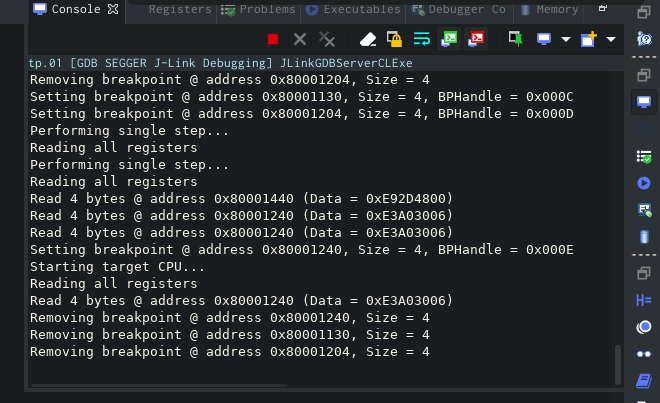
\includegraphics[width=.8\textwidth]{debug.png}
   \caption{Taille variables debugger}
\end{figure}

Pour la taille des variables, avec le debugger et la taille du code avec ls -la sur GNU/Linux

\paragraph{ Où se trouve chaque variable en mémoire (adresse absolue) ?}
\begin{itemize}
   \item value: 0x00F020E0
   \item gpio\_init: 0x8000e200
   \item banner: 0x8000e21c
   \item i: 0x800010C0
   \item lut: 0x800012A4 
   \item leds: 0x00F020E0
   \item msg: 0x8000e2ac
\end{itemize}
Nous avons trouvé sur le web que l'on pouvait avec l'opérateur \& afficher l'adresse d'une variable: printf("\%p\n", &x)

\paragraph{ Où se trouve le code en mémoire?}
Dans la heap, voir https://www.geeksforgeeks.org/memory-layout-of-c-program/

\paragraph{ Est-il possible d’améliorer / d’optimiser le code ? Si, oui comment ?}
Ayant très peu d'expérience avec C, nous avons pas trouvé comment le rendre plus efficace, nous avons émis une liste d'hypothèses:
      \begin{itemize}
         \item Limiter la taille ( au niveau du type choisi) des variables pour économiser de la place
         \item Contrôler qu'il n'y ait pas de memory leak
         \item Les boucles while infinie sont dangeureuse si tout à coup un problème survient sans pouvoir sortir
      \end{itemize}

\paragraph{Comment fonctonne de la macro ”ARRAY\_SIZE(x)”}
Il utilise la taille du en bytes du type choisit du tableau passé en paramètre et la divise avec la taille du type de son premier de son premier élément et permet de connaître le nombre d'élément dans un tableau. Dans ce code, le ARRAY\_SIZE est utilisé pour boucler à travers les GPIO


\section{Feedback}
Les questions étaient relativemment évasives et étant donnée que nous avions jamais eu de cours sur GIT ou C, il nous a fallu un peu de temps pour les appréhender. Nos réponses peuvent ne pas être correctes car nous sommes encore en train d'apprendre l'environnement dans lequel nous allons évoluer ces semestres

\end{document}
